\documentclass[10pt,a4paper]{article}
\usepackage[utf8]{inputenc}
\usepackage{amsthm, amsmath, mathtools, amssymb}
\usepackage[left=2cm,right=2cm,top=2cm,bottom=2cm]{geometry}
\usepackage[colorlinks,linkcolor=blue,citecolor=blue,urlcolor=blue]{hyperref}
\usepackage[catalan]{babel}
\usepackage{titlesec}
\usepackage{enumitem}
\usepackage{physics}
\usepackage{fancyhdr}
\usepackage{subcaption}
\usepackage{xcolor}
\usepackage{listings} 
\usepackage{parskip}

\allowdisplaybreaks % allow page breaks in align environment

\newcommand{\NN}{\ensuremath{\mathbb{N}}} % set of natural numbers
\newcommand{\ZZ}{\ensuremath{\mathbb{Z}}} % set of integers
\newcommand{\QQ}{\ensuremath{\mathbb{Q}}} % set of rationals
\newcommand{\RR}{\ensuremath{\mathbb{R}}} % set of real numbers
\newcommand{\CC}{\ensuremath{\mathbb{C}}} % set of complex numbers
\newcommand{\KK}{\ensuremath{\mathbb{K}}} % a general field

\newcommand{\vf}[1]{\boldsymbol{\mathrm{#1}}} % math style for vectors and matrices and vector-values functions (previously it was \*vb{#1} but this does not apply to greek letters)
\newcommand{\ii}{\mathrm{i}} % imaginary unit
\renewcommand{\O}[1]{\mathrm{O}\left(#1\right)} % big O-notation

\newtheorem{theorem}{Teorema}
\newtheorem{exercici}{Exercice}
\newtheorem{prop}{Proposició}
\theoremstyle{definition}
\newtheorem{definition}{Definició}
\theoremstyle{remark}
\newtheorem*{res}{Resolution}
\DeclareDocumentCommand\derivative{ s o m g d() }{ 
  % Total derivative
  % s: star for \flatfrac flat derivative
  % o: optional n for nth derivative
  % m: mandatory (x in df/dx)
  % g: optional (f in df/dx)
  % d: long-form d/dx(...)
    \IfBooleanTF{#1}
    {\let\fractype\flatfrac}
    {\let\fractype\frac}
    \IfNoValueTF{#4}
    {
        \IfNoValueTF{#5}
        {\fractype{\diffd \IfNoValueTF{#2}{}{^{#2}}}{\diffd #3\IfNoValueTF{#2}{}{^{#2}}}}
        {\fractype{\diffd \IfNoValueTF{#2}{}{^{#2}}}{\diffd #3\IfNoValueTF{#2}{}{^{#2}}} \argopen(#5\argclose)}
    }
    {\fractype{\diffd \IfNoValueTF{#2}{}{^{#2}} #3}{\diffd #4\IfNoValueTF{#2}{}{^{#2}}}\IfValueT{#5}{(#5)}}
} % differential operator
\DeclareDocumentCommand\partialderivative{ s o m g d() }{ 
  % Total derivative
  % s: star for \flatfrac flat derivative
  % o: optional n for nth derivative
  % m: mandatory (x in df/dx)
  % g: optional (f in df/dx)
  % d: long-form d/dx(...)
  \IfBooleanTF{#1}
    {\let\fractype\flatfrac}
    {\let\fractype\frac}
    \IfNoValueTF{#4}{
      \IfNoValueTF{#5}
      {\fractype{\partial \IfNoValueTF{#2}{}{^{#2}}}{\partial #3\IfNoValueTF{#2}{}{^{#2}}}}
      {\fractype{\partial \IfNoValueTF{#2}{}{^{#2}}}{\partial #3\IfNoValueTF{#2}{}{^{#2}}} \argopen(#5\argclose)}
    }
    {\fractype{\partial \IfNoValueTF{#2}{}{^{#2}} #3}{\partial #4\IfNoValueTF{#2}{}{^{#2}}}\IfValueT{#5}{(#5)}}
} % partial differential operator

\titleformat{\section}
  {\normalfont\fontsize{11}{15}\bfseries}{\thesection}{1em}{}

% \renewcommand{\theenumi}{\textbf{\arabic{enumi}}}
\renewcommand{\theenumi}{\alph{enumi}}
\renewcommand{\theenumiii}{\roman{enumiii}}
\renewcommand{\exp}[1]{\mathrm{e}^{#1}} % exponential function
\DeclareMathOperator*{\im}{Im}
\setlength\multlinegap{0pt} % disable the margins on \begin{multline} command.


  \definecolor{darkblue}{rgb}{0.0, 0.0, 0.55}

  \lstloadlanguages{C,Python,bash}
  \lstset{ %
          backgroundcolor=\color{white},   % choose the background color; you must add \usepackage{color} or \usepackage{xcolor}
          basicstyle=\color{red}\footnotesize\ttfamily,        % the size of the fonts that are used for the code
          breakatwhitespace=false,         % sets if automatic breaks should only happen at whitespace
          breaklines=true,                 % sets automatic line breaking
          captionpos=b,                    % sets the caption-position to bottom
          deletekeywords={...},            % if you want to delete keywords from the given language
          escapeinside={\%*}{*)},          % if you want to add LaTeX within your code
          extendedchars=true,              % lets you use non-ASCII characters; for 8-bits encodings only, does not work with UTF-8
          frame=single,                    % adds a frame around the code
          keepspaces=true,                 % keeps spaces in text, useful for keeping indentation of code (possibly needs columns=flexible)
          keywordstyle=\color{darkblue},       % keyword style
          commentstyle=\itshape\color{gray},
          identifierstyle=\color{black},
          language=C,                 % the language of the code
          otherkeywords={*,...},           % if you want to add more keywords to the set
          numbers=left,                    % where to put the line-numbers; possible values are (none, left, right)
          numbersep=5pt,                   % how far the line-numbers are from the code
          numberstyle=\tiny\color{gray}, % the style that is used for the line-numbers
          rulecolor=\color{gray},         % if not set, the frame-color may be changed on line-breaks within not-black text (e.g. comments (green here))
          showspaces=false,                % show spaces everywhere adding particular underscores; it overrides 'showstringspaces'
          showstringspaces=false,          % underline spaces within strings only
          showtabs=false,                  % show tabs within strings adding particular underscores
          stepnumber=1,                    % the step between two line-numbers. If it's 1, each line will be numbered
          stringstyle=\color{blue},     % string literal style
          tabsize=2,                         % sets default tabsize to 2 spaces
          %title=\lstname                   % show the filename of files included with \lstinputlisting; also try caption instead of title
  }
  \lstset{literate=
          {á}{{\'a}}1 {é}{{\'e}}1 {í}{{\'i}}1 {ó}{{\'o}}1 {ú}{{\'u}}1
          {Á}{{\'A}}1 {É}{{\'E}}1 {Í}{{\'I}}1 {Ó}{{\'O}}1 {Ú}{{\'U}}1
          {à}{{\`a}}1 {è}{{\`e}}1 {ì}{{\`i}}1 {ò}{{\`o}}1 {ù}{{\`u}}1
          {À}{{\`A}}1 {È}{{\'E}}1 {Ì}{{\`I}}1 {Ò}{{\`O}}1 {Ù}{{\`U}}1
          {ä}{{\"a}}1 {ë}{{\"e}}1 {ï}{{\"i}}1 {ö}{{\"o}}1 {ü}{{\"u}}1
          {Ä}{{\"A}}1 {Ë}{{\"E}}1 {Ï}{{\"I}}1 {Ö}{{\"O}}1 {Ü}{{\"U}}1
          {â}{{\^a}}1 {ê}{{\^e}}1 {î}{{\^i}}1 {ô}{{\^o}}1 {û}{{\^u}}1
          {Â}{{\^A}}1 {Ê}{{\^E}}1 {Î}{{\^I}}1 {Ô}{{\^O}}1 {Û}{{\^U}}1
          {œ}{{\oe}}1 {Œ}{{\OE}}1 {æ}{{\ae}}1 {Æ}{{\AE}}1 {ß}{{\ss}}1
          {ű}{{\H{u}}}1 {Ű}{{\H{U}}}1 {ő}{{\H{o}}}1 {Ő}{{\H{O}}}1
          {ç}{{\c c}}1 {Ç}{{\c C}}1 {ø}{{\o}}1 {å}{{\r a}}1 {Å}{{\r A}}1
          {€}{{\EUR}}1 {£}{{\pounds}}1
  }

\title{\bfseries\Large Control discret de trajectòries mitjançant maniobres impulsives}

\author{Víctor Ballester Ribó\\NIU: 1570866}
\date{\parbox{\linewidth}{\centering
  Càlcul numèric\endgraf
  Grau en Matemàtiques\endgraf
  Universitat Autònoma de Barcelona\endgraf
  Juny de 2023}}
  \pagestyle{fancy}
  \fancyhf{}
  \fancyhfoffset[L]{1cm}
  \fancyhfoffset[R]{1cm}
  \rhead{NIU: 1570866}
  \lhead{Víctor Ballester}
  \cfoot{\thepage}
  %\setlength{\headheight}{13.6pt}

\setlength{\parindent}{0pt}
\begin{document}
\selectlanguage{catalan}
\maketitle
L'objectiu d'aquesta pràctica és resoldre el problema de calcular maniobres per impulsar un satè\lgem it, des d'una posició i velocitat fins a unes altres. Per això primer farem diversos problemes d'exemple.

Abans de tot, per a el correcte ús del codi, cal donar permisos d'execució al fitxer \texttt{execute.sh}\footnote{Totes les instruccions que apareixen en aquest document són vàlides per a sistemes UNIX. Per a sistemes Windows, podrien variar lleugerament.}:
\begin{lstlisting}[language=Bash]
chmod +x execute.sh
\end{lstlisting}
\section*{Part 1}
Considerem el sistema diferencial que modela el moviment d'un pèndol forçat i amb fregament.
$$
  \begin{cases}
    \dot{r} = v \\
    \dot{v} = -\sin r - \mu v + \sin(\omega t)
  \end{cases}
$$
on $\mu,\omega\geq 0$. Si executem el codi amb
\begin{lstlisting}[language=Bash]
./execute.sh pendulum
\end{lstlisting}
obtindrem el següent gràfic, on es mostren diverses òrbites del sistema:
\begin{figure}[ht]
  \centering
  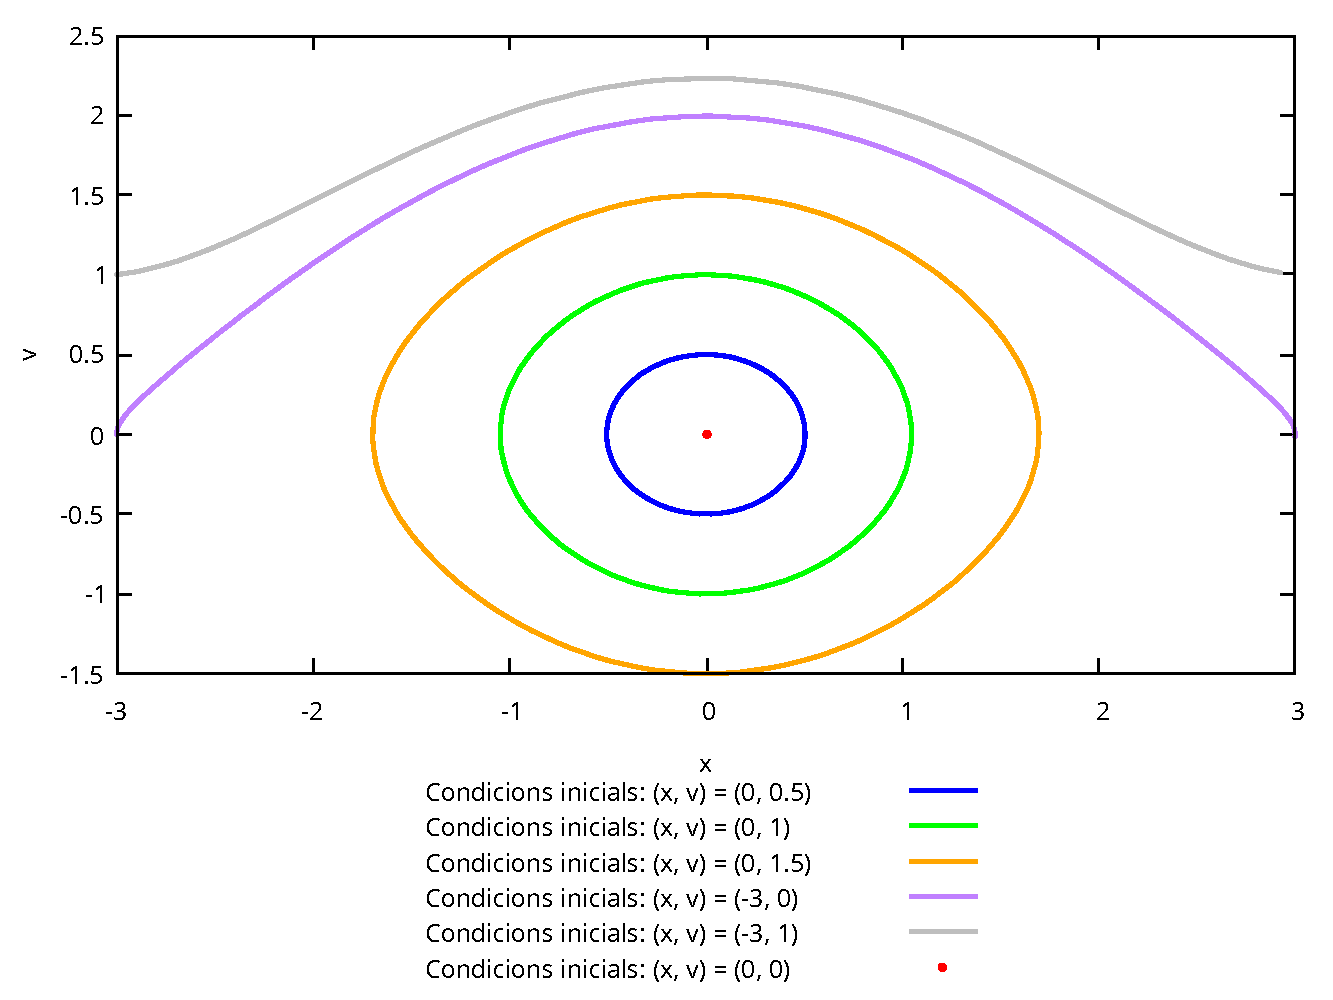
\includegraphics[width=0.69\linewidth]{Images/pendulum.pdf}
  \caption{Òrbites del sistema del pèndol amb $\mu=0$ i $\omega=0$ partint de diversos punts inicials.}
\end{figure}

Ara considerem els següents problemes d'equacions diferencials:
$$
  \begin{cases}
    y'=2 y/t \\
    y(1)=1
  \end{cases}\qquad
  \begin{cases}
    x'=y  \\
    y'=-x \\
    x(0)=1, y(0)=1
  \end{cases}
$$
Les solucions d'aquests dos problemes són fàcils d'obtenir i venen donades respectivament per:
$$
  y(t)=t^2\qquad x(t)=\cos t + \sin t
$$
L'objectiu d'aquesta part de la pràctica és calcular el flux d'aquests dos sistemes diferencials en el punt $t=2$ i $t=1$, respectivament. Executant
\begin{lstlisting}[language=Bash]
./execute.sh flow_sample
\end{lstlisting}
observem que els valors obtinguts són idèntics als reals: $y(2)=4$ i $x(1)=\cos 1 + \sin 1\simeq 1.3817732907$.

Considerem ara el sistema de Lorenz:
$$
  \begin{cases}
    x'=\sigma(y-x)     \\
    y'=\rho x - y - xz \\
    z'=-\beta z + xy
  \end{cases}
$$
amb $\sigma=10$, $\rho=28$ i $\beta=2.6$. Si executem
\begin{lstlisting}[language=Bash]
./execute.sh lorenz
\end{lstlisting}
obtindrem el següent gràfic:
\begin{figure}[ht]
  \centering\vspace{-2cm}
  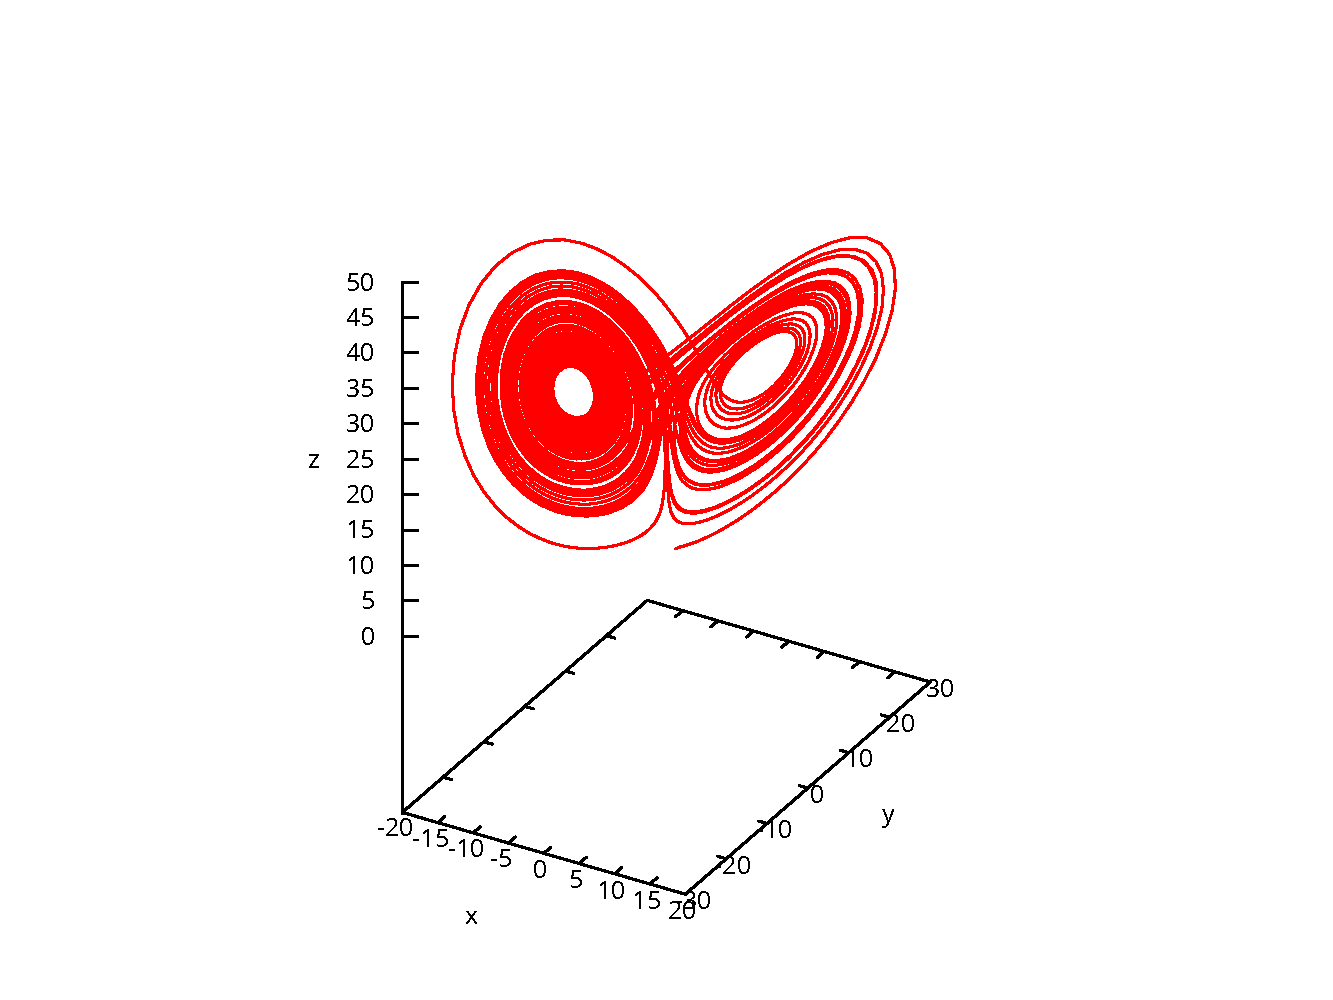
\includegraphics[width=0.7\linewidth]{Images/lorenz.pdf}
  \caption{Òrbita del sistema de Lorenz partint de $(1.1,0.36,3.14)$.}
\end{figure}

Finalment, considerem el problema restringit dels tres cossos. En coordenades sinòdiques, el sistema ve donat per:
$$
  \begin{cases}
    \vf{\dot{r}} = \vf{v} \\
    \vf{\dot{v}} = \vf{a}
  \end{cases}
$$
on
\begin{align*}
  \vf{r}         & ={(x,y,z)}^\mathrm{T}                                                              \\
  \vf{v}         & ={(u,v,w)}^\mathrm{T}                                                              \\
  \vf{a}         & =2{(v,-u,0)}^\mathrm{T}+\grad\Omega(\vf{r})                                        \\
  \Omega(\vf{r}) & =\frac{x^2+y^2}{2} + \frac{1-\mu}{\rho_1}+\frac{\mu}{\rho_2}-\frac{1}{2}\mu(1-\mu) \\
  \rho_1         & =\sqrt{{(x-\mu)}^2+y^2+z^2}                                                        \\
  \rho_2         & =\sqrt{{(x+1-\mu)}^2+y^2+z^2}                                                      \\
  \mu            & =\frac{m_1}{m_1+m_2}
\end{align*}
assumint $m_1\geq m_2$. Si executem
\begin{lstlisting}[language=Bash]
./execute.sh rtbps
\end{lstlisting}
obtindrem el següent gràfic:
\begin{figure}[ht]
  \centering\vspace{-2cm}
  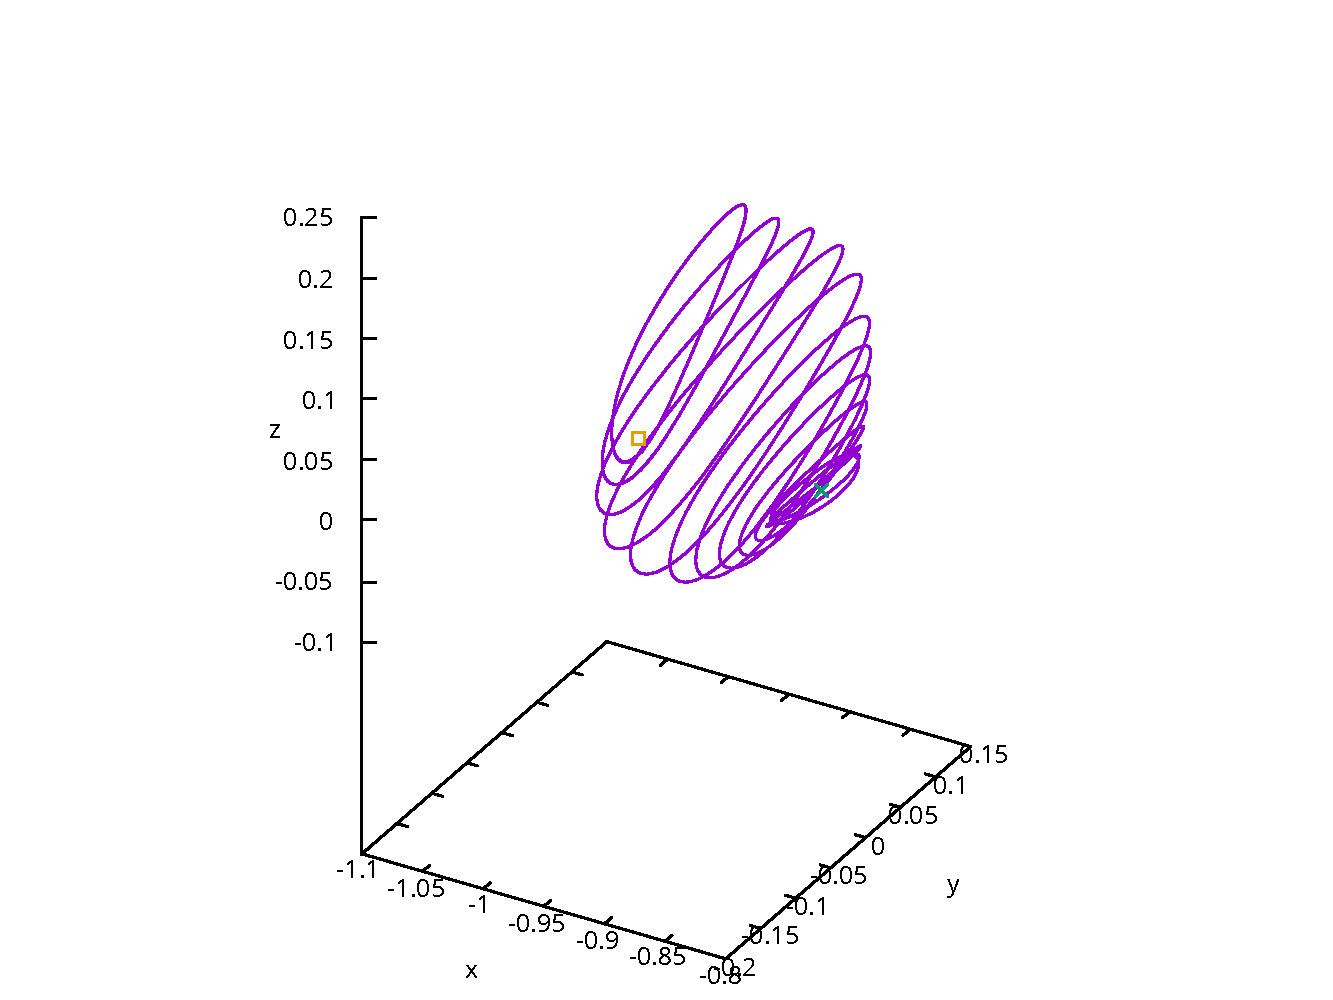
\includegraphics[width=0.7\linewidth]{Images/rtbps.pdf}
  \caption{Continu d'òrbites periòdiques del sistema del problema restringit de 3 cossos. El quadrat groc correspon a la lluna i la creu blava al punt d'equilibri de Lagrange $L_1$. No hem dibuixat la Terra, situada en $(0.01215, 0, 0)$, perquè distorsionava la mida de la imatge.}
\end{figure}
\section*{Part 2}
En aquesta part de la pràctica l'objectiu és implementar el càlcul de la diferencial del flux d'un sistema diferencial. Per a comprovar que el que hem fet és el correcte, compararem els valors numèrics de les derivades del flux mitjançant dos mètodes: a partir de les variacionals i calculant la derivada com una diferència finita centrada. Per a fer-ho, considerarem el següent sistema diferencial:
$$
  \begin{cases}
    x'=\alpha (1 - r^2)x -y \\
    y'=x+\alpha (1 - r^2)y
  \end{cases}
$$
on $r^2=x^2+y^2$. Si executem
\begin{lstlisting}[language=Bash]
./execute.sh ex2
\end{lstlisting}
obtindrem els següents erros entre els valors numèrics de les derivades del flux (usant una tolerància de $10^{-6}$ per Runge-Kutta i de $10^{-4}$ per la diferència finita centrada):
\begin{align*}
  \phi^1_x & \to 5.40878\times 10^{-11} \\
  \phi^1_y & \to 3.15831\times 10^{-10} \\
  \phi^2_x & \to 5.04729\times 10^{-10} \\
  \phi^2_y & \to 3.9809\times 10^{-10}
\end{align*}
on el $\vf\phi=(\phi^1,\phi^2)$ és el flux del sistema.
\section*{Part 4}
En aquesta última part de la pràctica l'objectiu és trobar les maniobres $\Delta \vf{v}_0$ i $\Delta \vf{v}_1$ que permeten passar d'una posició i velocitat inicials ${(\vf{r}_0,\vf{v}_0)}^\mathrm{T}$ donades a una posició i velocitat finals ${(\vf{r}_f,\vf{v}_f)}^\mathrm{T}$ també donades, en un temps $\Delta t$. Més precisament, volem trobar maniobres que permetin fer el següent:
\begin{align*}
  \begin{pmatrix}
    \vf{r}_0 \\
    \vf{v}_0
  \end{pmatrix} & \overset{\substack{\text{maniobra}   \\\Delta\vf{v}_0}}{\longrightarrow}
  \begin{pmatrix}
    \vf{r}_0 \\
    \vf{v}_0 + \Delta\vf{v}_0
  \end{pmatrix}                             \\ & \overset{\text{vol lliure}}{\longrightarrow}\vf\phi_{\Delta t/2}\begin{pmatrix}
    \vf{r}_0 \\
    \vf{v}_0 + \Delta\vf{v}_0
  \end{pmatrix}\\
                  & \overset{\substack{\text{maniobra} \\\Delta\vf{v}_1}}{\longrightarrow}
  \vf\phi_{\Delta t/2}\begin{pmatrix}
                        \vf{r}_0 \\
                        \vf{v}_0 + \Delta\vf{v}_0
                      \end{pmatrix}+\begin{pmatrix}
                                      \vf{0} \\
                                      \Delta\vf{v}_1
                                    \end{pmatrix}     \\ & \overset{\text{vol lliure}}{\longrightarrow}\vf\phi_{\Delta t/2}\left(\phi_{\Delta t/2}\begin{pmatrix}
    \vf{r}_0 \\
    \vf{v}_0 + \Delta\vf{v}_0
  \end{pmatrix}+\begin{pmatrix}
    \vf{0} \\
    \Delta\vf{v}_1
  \end{pmatrix}\right)
\end{align*}
Per tant, cal trobar $\Delta\vf{v}={(\Delta\vf{v}_0,\Delta\vf{v}_1)}^\mathrm{T}$ tal que anu\lgem in la funció:
$$
  \vf{G}(\Delta\vf{v}) = \vf\phi_{\Delta t/2}\left(\phi_{\Delta t/2}\begin{pmatrix}
    \vf{r}_0 \\
    \vf{v}_0 + \Delta\vf{v}_0
  \end{pmatrix}+\begin{pmatrix}
    \vf{0} \\
    \Delta\vf{v}_1
  \end{pmatrix}\right) - \begin{pmatrix}
    \vf{r}_f \\
    \vf{v}_f
  \end{pmatrix}
$$
Això ho resoldrem mitjançant el mètode de Newton multidimensional. Per a fer-ho, necessitem calcular la matriu jacobiana de $\vf{G}$, que ho podrem fer a partir de les variacionals del flux. Per a trobar els iterats de Newton, usarem el mètode de Gauss per resoldre el sistema lineal associat.

Comencem primer amb un problema d'exemple, el del pèndol. Suposem que $r_0=1$, $v_0=0$, $r_f=0$, $v_f=-\sqrt{2(1-\cos 1)}
  \simeq -0.95885108$ i $\Delta t=\pi/2$. Si executem la instrucció
\begin{lstlisting}[language=Bash]
./execute.sh ex43
\end{lstlisting}
obtindrem el següent resultat:
$$
  \Delta\vf{v} = \begin{pmatrix}
    -0.0926981627735679 \\
    0.0062078732568572
  \end{pmatrix}
$$
amb una tolerància de $10^{-12}$.

Finalment, si executem la instrucció
\begin{lstlisting}[language=Bash]
./execute.sh cmani_rtbp
\end{lstlisting}
obtindrem que les maniobres necessàries per passar del punt inicial
$$
  \begin{pmatrix}
    {\vf{r}_0}^\mathrm{T} \\
    {\vf{v}_0}^\mathrm{T}
  \end{pmatrix} =
  \begin{pmatrix}
    -0.8457719086638686 & 0.05934028672713117 & 0                   \\
    0.03769526738828564 & 0.01515062570613701 & 0.04577799834681743
  \end{pmatrix}
$$ al punt final
$$
  \begin{pmatrix}
    {\vf{r}_f}^\mathrm{T} \\
    {\vf{v}_f}^\mathrm{T}
  \end{pmatrix}=
  \begin{pmatrix}
    -0.8518851062423166 & 0.06132143191581388 & 0.0005120725158794939 \\
    0.0206128163364461  & 0.01844596878578819 & 0.04641615142301939
  \end{pmatrix}
$$ en un temps $\Delta t = 2.746177778348061$ són:
$$
  \begin{pmatrix}
    {\Delta\vf{v}_0}^\mathrm{T} \\
    {\Delta\vf{v}_1}^\mathrm{T}
  \end{pmatrix}=\begin{pmatrix}
    -8.326184791197963\times10^{-6} & -1.285657562239232\times10^{-5} & -1.545884623736697\times10^{-6} \\
    -5.989126097485234\times10^{-6} & -1.071156972197014\times10^{-5} & -1.809272933729815\times10^{-6}
  \end{pmatrix}
$$
\end{document}